\documentclass[titlepage]{article}
\usepackage{graphicx}       % include figures
\usepackage{float}          % align figures
\usepackage{amsmath}        % \pm
% \usepackage{indentfirst}
\usepackage{achemso}
\usepackage[bf]{caption}    % bold figure names
\usepackage{url}
\usepackage{setspace}
\restylefloat{table}        % same page tables
\usepackage{chngpage}
\usepackage{multirow}

\begin{document}




\title{Application of Machine Learning Methods to the Optoelectronic properties of Benzobisazoles}
\author{Christopher Collins}

\maketitle

\doublespace
\section{Introduction}

Organic solar cell stuff, cruiform stuff, machine learning stuff

\section{Naming Scheme}

The naming scheme is broken down into three separate components. These parts are the core, the sides, and the options.

\begin{figure}[H]
  \begin{center}
    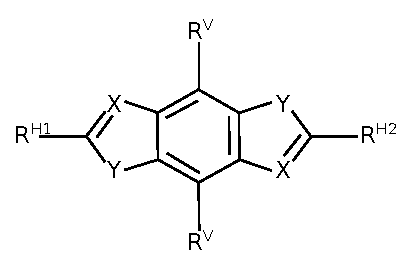
\includegraphics[width=1.25in]{TXY.eps}
  \end{center}
  \caption{TXY Core}
  \label{fig:txy}
\end{figure}



The core is the central part of the molecule. All cores are identified by a combination of three letters. The first letter indicates whether or not the structure is Cis or Trans which correspond to the letters C and T respectively. The second letter in the core name is the symbol for the element that is in the core without the $\pi$ bond (meh?) (for consistency in naming this will always be the top right atom). This can be one of O, S, N, P, or C. The final letter is the remaining element's symbol which can be N, P, or C (for consistency this will always be the bottom right atom).

\begin{figure}[H]
  \begin{center}
    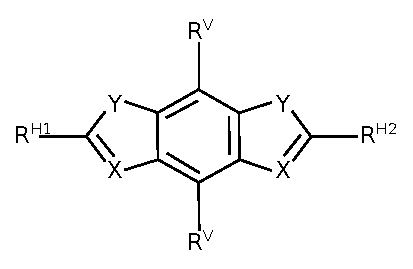
\includegraphics[width=1.25in]{CXY.eps}
  \end{center}
  \caption{CXY Core}
  \label{fig:cxy}
\end{figure}

The sides of the name are split into three groups based on the location in the structure. Going from the core orientation, these three groups are the left, center, and right sides. The left and right sides of the structure form the horizontal axis. The center group is the vertical axis and ... something about how they are the same....

\begin{table}[H]
  \centering
  \caption{Aryl Groups}
  \begin{tabular}{ccc}
    Label   & Name          & Structure \\
    \hline
    2       & Double Bond   &           \\
    3       & Triple Bond   &           \\
    4       & Phenyl        &           \\
    5       & Thiophene     &           \\
    6       & Pyridine      &           \\
    7       & Carbazole     &           \\
    8       & TZ            &           \\
    9       & EDOT          &           \\
    \hline
  \end{tabular}
  \label{tab:aryl}
\end{table}

Each side is then broken down into components of Aryl, X, and R groups. Aryl groups are indicated by the numbers 2 through 9 as seen in Table \ref{tab:aryl}. Aryl groups form the main chain part of the structure...

\begin{table}[H]
  \centering
  \caption{X/R-Groups}
  \begin{tabular}{ccc}
    Label   & Name          & Structure \\
    \hline
    A/a     & Hydrogen  &           \\
    B/b     & Chlorine  &           \\
    C/c     & Bromine   &           \\
    D/d     & CN        &           \\
    E/e     & CCH       &           \\
    F/f     & OH        &           \\
    G/g     & SH        &           \\
    H/h     & $NH_2$    &           \\
    I/i     & $CH_3$    &           \\
    J/j     & Phenyl    &           \\
    K/k     & TMS       &           \\
    L/l     & $OCH_3$   &           \\
    *       & Spacer    &           \\
    \hline
  \end{tabular}
  \label{tab:xrgroups}
\end{table}


X and R groups are both composed of the same set of substituents seen in TABLE 2. X groups are the letters A through L, and r groups are a through l. The main difference between X and R groups is where they are placed in the chain, whereas R-Groups are placed on the Aryl group that directly proceeds them. As can be seen in TABLE 1 R-groups come in pairs of two. These groups can either be the same or different(?). Because there are some Aryl groups that do not allow any R-groups there is an additional spacer R-group that is designated as *. It has no effect on the structure of the molecule, it is just used as a place holder when converting the names to a feature vector.


Starting from the core going outward, side chains take two main forms. They are either an X-group (which terminates the entire side) or they are a triplet of an Aryl group and two R-groups. If it is an aryl group triplet, then the process can continue.
(X-group|[Aryl, R-group, R-group])


The final component of the naming scheme is a set of options. These are broken up into two main classes. The first pair of options are the polymer options and they indicate how many times the molecules is repeated along the horizontal (n) axis (chain?) or the vertical (m) axis (chain?). The second set of options is a set of x, y, and z that are the number of times that the molecule is stacked in each direction(?).



Structures were picked using this naming scheme to try to cover as many combinations of cores, sides, and options.


\section{Feature Vectors}

Using this naming scheme, it is apparent that there are multiple ways that these could be converted into feature vectors for use in machine learning.

\subsection{Naive}
The first, and most simplistic, is to take all the possible options ....
The problem with this approach is that is the size of the feature vector groups proportional to the length of the longest side chain. Another problem with this type of feature vector it does not exploit similarities in the structure. (one might expect a chlorine two steps away from the core to cause about the same effect as one one step away times some decay factor).


\subsection{Decay}
To counter act these problems a second feature vector was created that used a decay function \eqref{decay}. $A$, $H$, and $p$ are arbitrary constants used to adjust the decay. By grouping similar components together (?), it normalizes implict features by ... something (charge, hammet parameters).

\begin{equation}\label{decay}
    Value = \sum_i^n (A d_i^{-H})^{p}
\end{equation}

The bad thing about this kind of decay function is that it is not separable if $H \times p \le 1$. This would mean that there is no unique conversion between a given feature vector and its associated name/structure.

\subsection{Decay with Length Corrections}

One problem with the first decay type feature vector is it makes the assumption that all the distances between are the same length. Since the effects of atoms are highly dependent on distance this sort of assumption is problematic for heterogeneous side groups. \eqref{decay2} Something something. This normalizes all the lengths such that longer structures will increase the distance more than shorter structures.

$\vec L$ is a vector of the length from the first primary connector to the second for all the Aryl groups. Using this vector, a ratio matrix is constructed such that $R_{ij} = \vec L_j / \vec L_i$. By doing this, all the lengths are normalized relative ??.
$$\textbf{R} = \vec L / \vec L^{T}$$
$$ \vec d = \sum_{i,j}^n \textbf{R}_{ij}  $$
\begin{equation}\label{decay2}
    Value = \sum_i^n (A d_i^{-H})^{p}
\end{equation}

The problem with this feature vector is that it is not separable.

\subsection{Decay with Predictions}

In attempt to exploit the relation between HOMO, LUMO, and Band Gap, another feature vector was constructed. The feature vector was composed of a combination of the decay vector plus the addition of the two properties that were not being trained for.

$$ predictedHOMO = predict(Decay, HOMO) $$
$$ predictedLUMO = predict(Decay, LUMO) $$
$$ predictedGAP = predict(Decay, GAP) $$
$$ GAPit = [Decay, predictedHOMO, predictedLUMO] $$
$$ HOMOit = [Decay, predictedLUMO, predictedGAP] $$
$$ LUMOit = [Decay, predictedGAP, predictedHOMO] $$

\section{Methods}
\subsection{Mean Value}
\subsection{Linear Regression}
\subsubsection{Regular}
\subsubsection{Ridged}
\subsection{Tree}
\subsection{k-Nearest Neighbors}
\subsection{Support Vector Machines}

% \begin{figure}[H]
%   \begin{center}
%     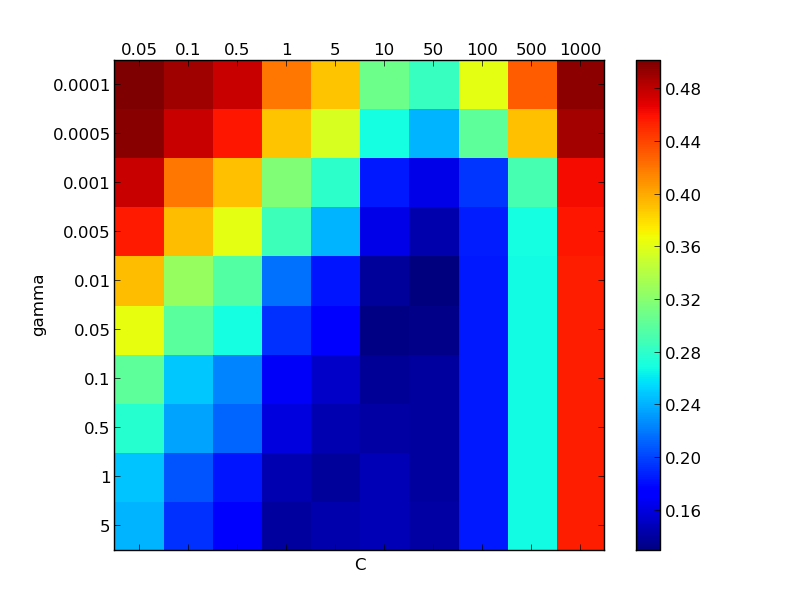
\includegraphics[width=5in]{scan2.png}
%   \end{center}
%   \caption{Scan of SVM parameters C and gamma}
%   \label{fig:homolumo}
% \end{figure}

\subsubsection{Gaussian Kernel}
$$ k(x, x') = exp\left( −\frac{1}{2\sigma^2} \lVert x - x'  \rVert^2 \right) $$

\subsubsection{Laplacian Kernel}
$$ k(x, x') = exp\left( −\frac{1}{\sigma} \lvert x - x' \rvert \right) $$


\section{Procedure}

Roughly 1100 benzobisazole structures were built (using a script?). Once they were built the structures were optimized using Density Functional Theory (DFT) with B3LYP/6-31(g). After the optimization, the molecules were then ran with Time Dependent Density Functional Theory (TDDFT) with B3LYP/6-31(g).

Beyond the 1100 benzobisazole structures, about 1000 other structures were collected for comparison (?).

Once all the calculations were completed, the resulting log files were parsed for HOMO, LUMO, and Band Gap values. From there, the first three feature vectors were constructed (Naive, Decay, Decay with Distance Correction) and the resulting vectors were stored with the parsed log data.

(When to mention Decay with Prediction creation?)

Once all the data and feature vectors were collected, the machine learning stuff...

For each feature vector, property, method set the methods relevant parameters were optimized (C, gamma, max depth, alpha, n neighbors). Then using these optimized parameters, the machine learning models were trained using k-folds specifically using 10 folds (bla bla).

(maybe invert the procedure)

\section{Results}

\begin{table}[H]
  \centering
  \caption{Band Gap Results}
  \begin{tabular}{lll}
            Feature Vector     & Method       & MAE (eV)                \\
    \hline\hline
    \multirow{7}{*}{Naive}     & Mean Value   & 0.5051 $\pm$ 0.044 \\
                               & Linear       & 0.2628 $\pm$ 0.019 \\
                               & Linear Ridge & 0.2571 $\pm$ 0.020 \\
                               & Tree         & 0.1429 $\pm$ 0.016 \\
                               & k-NN         & 0.2096 $\pm$ 0.018 \\
                               & SVM Gauss    & \textbf{0.1355 $\pm$ 0.011} \\
                               & SVM Laplace  & 0.1681 $\pm$ 0.013 \\
    \hline
    \multirow{7}{*}{Decay}     & Mean Value   & 0.5051 $\pm$ 0.044 \\
                               & Linear       & 0.2531 $\pm$ 0.022 \\
                               & Linear Ridge & 0.2506 $\pm$ 0.023 \\
                               & Tree         & 0.1318 $\pm$ 0.018 \\
                               & k-NN         & 0.2112 $\pm$ 0.017 \\
                               & SVM Gauss    & \textbf{0.1297 $\pm$ 0.011} \\
                               & SVM Laplace  & 0.1591 $\pm$ 0.011 \\
    \hline
    \multirow{7}{*}{Decay with Length Corrections} & Mean Value   & 0.5051 $\pm$ 0.044 \\
                               & Linear       & 0.2485 $\pm$ 0.020 \\
                               & Linear Ridge & 0.2466 $\pm$ 0.020 \\
                               & Tree         & 0.1492 $\pm$ 0.029 \\
                               & k-NN         & 0.2169 $\pm$ 0.013 \\
                               & SVM Gauss    & \textbf{0.1314 $\pm$ 0.011} \\
                               & SVM Laplace  & 0.1631 $\pm$ 0.011 \\
    \hline
    \multirow{7}{*}{Decay with Predictions} & Mean Value   & 0.5051 $\pm$ 0.044 \\
                               & Linear       & 0.1211 $\pm$ 0.011 \\
                               & Linear Ridge & 0.1174 $\pm$ 0.010 \\
                               & Tree         & 0.1369 $\pm$ 0.012 \\
                               & k-NN         & 0.1724 $\pm$ 0.015 \\
                               & SVM Gauss    & \textbf{0.1004 $\pm$ 0.010} \\
                               & SVM Laplace  & 0.1154 $\pm$ 0.009 \\
    \hline\hline
  \end{tabular}
  \label{tab:gapresults}
\end{table}



% dummy           0.5051634571 $\pm$ 0.0445987177
% linear          0.2628013865 $\pm$ 0.0191410131
% linear ridge    0.2571941447 $\pm$ 0.0201764172
% tree            0.1429020978 $\pm$ 0.0167680834
% neighbors       0.2096637025 $\pm$ 0.0181147991
% svm gauss       0.1355760073 $\pm$ 0.0119249721
% svm laplace     0.1681324515 $\pm$ 0.0130277607

% dummy           0.5051634571 $\pm$ 0.0445987177
% linear          0.2531408695 $\pm$ 0.0224904198
% linear ridge    0.2506620918 $\pm$ 0.0231378900
% tree            0.1318830228 $\pm$ 0.0188910719
% neighbors       0.2112675515 $\pm$ 0.0170114767
% svm gauss       0.1297476028 $\pm$ 0.0110853891
% svm laplace     0.1591951178 $\pm$ 0.0113296220

% dummy           0.5051634571 $\pm$ 0.0445987177
% linear          0.2485031607 $\pm$ 0.0200054080
% linear ridge    0.2466766131 $\pm$ 0.0209252773
% tree            0.1492425133 $\pm$ 0.0293509142
% neighbors       0.2169500774 $\pm$ 0.0136509896
% svm gauss       0.1314727141 $\pm$ 0.0116959757
% svm laplace     0.1631757401 $\pm$ 0.0117913187

% dummy           0.5051634571 $\pm$ 0.0445987177
% linear          0.1211359604 $\pm$ 0.0116286996
% linear ridge    0.1174973321 $\pm$ 0.0101995097
% tree            0.1369228897 $\pm$ 0.0123968003
% neighbors       0.1724752783 $\pm$ 0.0152423160
% svm gauss       0.1004123381 $\pm$ 0.0106025428
% svm laplace     0.1154254876 $\pm$ 0.0096740880


\begin{table}[H]
  \centering
  \caption{HOMO Results}
  \begin{tabular}{lll}
            Feature Vector     & Method       & MAE (eV)                \\
    \hline\hline
    \multirow{7}{*}{Naive} & Mean Value   & 0.4330 $\pm$ 0.038 \\
                               & Linear       & 0.2002 $\pm$ 0.024 \\
                               & Linear Ridge & 0.1949 $\pm$ 0.024 \\
                               & Tree         & 0.1546 $\pm$ 0.012 \\
                               & k-NN         & 0.2449 $\pm$ 0.025 \\
                               & SVM Gauss    & \textbf{0.1126 $\pm$ 0.014} \\
                               & SVM Laplace  & 0.1557 $\pm$ 0.016 \\
    \hline
    \multirow{7}{*}{Decay}     & Mean Value   & 0.4330 $\pm$ 0.038 \\
                               & Linear       & 0.1868 $\pm$ 0.025 \\
                               & Linear Ridge & 0.1860 $\pm$ 0.025 \\
                               & Tree         & 0.1455 $\pm$ 0.017 \\
                               & k-NN         & 0.2549 $\pm$ 0.026 \\
                               & SVM Gauss    & \textbf{0.1069 $\pm$ 0.010} \\
                               & SVM Laplace  & 0.1431 $\pm$ 0.014 \\
    \hline
    \multirow{7}{*}{Decay with Length Corrections} & Mean Value   & 0.4330 $\pm$ 0.038 \\
                               & Linear       & 0.1883 $\pm$ 0.024 \\
                               & Linear Ridge & 0.1875 $\pm$ 0.025 \\
                               & Tree         & 0.1453 $\pm$ 0.021 \\
                               & k-NN         & 0.2622 $\pm$ 0.028 \\
                               & SVM Gauss    & \textbf{0.1082 $\pm$ 0.012} \\
                               & SVM Laplace  & 0.1457 $\pm$ 0.017 \\
    \hline
    \multirow{7}{*}{Decay with Predictions} & Mean Value   & 0.4330 $\pm$ 0.038 \\
                               & Linear       & 0.0904 $\pm$ 0.007 \\
                               & Linear Ridge & 0.0897 $\pm$ 0.008 \\
                               & Tree         & 0.1439 $\pm$ 0.016 \\
                               & k-NN         & 0.1734 $\pm$ 0.020 \\
                               & SVM Gauss    & \textbf{0.0852 $\pm$ 0.007} \\
                               & SVM Laplace  & 0.1001 $\pm$ 0.008 \\
    \hline\hline
  \end{tabular}
  \label{tab:gapresults}
\end{table}

% dummy            0.4330672042 $\pm$ 0.0380947474
% linear           0.2002858544 $\pm$ 0.0244903400
% linear ridge     0.1949752271 $\pm$ 0.0248602704
% tree             0.1546552205 $\pm$ 0.0122826022
% neighbors        0.2449855565 $\pm$ 0.0258103540
% svm gauss        0.1126612407 $\pm$ 0.0141583310
% svm laplace      0.1557953600 $\pm$ 0.0169683266

% dummy            0.4330672042 $\pm$ 0.0380947474
% linear           0.1868573168 $\pm$ 0.0252679509
% linear ridge     0.1860609806 $\pm$ 0.0257993800
% tree             0.1455811816 $\pm$ 0.0175405978
% neighbors        0.2549135699 $\pm$ 0.0261735083
% svm gauss        0.1069055686 $\pm$ 0.0100414699
% svm laplace      0.1431763121 $\pm$ 0.0145504211

% dummy            0.4330672042 $\pm$ 0.0380947474
% linear           0.1883473946 $\pm$ 0.0248143868
% linear ridge     0.1875977704 $\pm$ 0.0251635444
% tree             0.1453857318 $\pm$ 0.0214142873
% neighbors        0.2622268718 $\pm$ 0.0287591181
% svm gauss        0.1082111822 $\pm$ 0.0124536000
% svm laplace      0.1457133829 $\pm$ 0.0170146564

% dummy            0.4330672042 $\pm$ 0.0380947474
% linear           0.0904848003 $\pm$ 0.0077179117
% linear ridge     0.0897196018 $\pm$ 0.0085006159
% tree             0.1439614181 $\pm$ 0.0167746654
% neighbors        0.1734307394 $\pm$ 0.0202218099
% svm gauss        0.0852044604 $\pm$ 0.0072159851
% svm laplace      0.1001281598 $\pm$ 0.0086522943

\begin{table}[H]
  \centering
  \caption{LUMO Results}
  \begin{tabular}{lll}
            Feature Vector     & Method       & MAE (eV)                \\
    \hline\hline
    \multirow{7}{*}{Naive}     & Mean Value   & 0.4475 $\pm$ 0.037 \\
                               & Linear       & 0.1900 $\pm$ 0.028 \\
                               & Linear Ridge & 0.1862 $\pm$ 0.025 \\
                               & Tree         & 0.1529 $\pm$ 0.007 \\
                               & k-NN         & 0.2351 $\pm$ 0.019 \\
                               & SVM Gauss    & \textbf{0.1055 $\pm$ 0.010} \\
                               & SVM Laplace  & 0.1454 $\pm$ 0.014 \\
    \hline
    \multirow{7}{*}{Decay}     & Mean Value   & 0.4475 $\pm$ 0.037 \\
                               & Linear       & 0.1816 $\pm$ 0.026 \\
                               & Linear Ridge & 0.1801 $\pm$ 0.026 \\
                               & Tree         & 0.1510 $\pm$ 0.024 \\
                               & k-NN         & 0.2323 $\pm$ 0.017 \\
                               & SVM Gauss    & \textbf{0.1022 $\pm$ 0.015} \\
                               & SVM Laplace  & 0.1317 $\pm$ 0.012 \\
    \hline
    \multirow{7}{*}{Decay with Length Corrections} & Mean Value   & 0.4475 $\pm$ 0.037 \\
                               & Linear       & 0.1847 $\pm$ 0.027 \\
                               & Linear Ridge & 0.1828 $\pm$ 0.027 \\
                               & Tree         & 0.1540 $\pm$ 0.023 \\
                               & k-NN         & 0.2348 $\pm$ 0.014 \\
                               & SVM Gauss    & \textbf{0.1029 $\pm$ 0.012} \\
                               & SVM Laplace  & 0.1331 $\pm$ 0.012 \\
    \hline
    \multirow{7}{*}{Decay with Predictions} & Mean Value   & 0.4475 $\pm$ 0.037 \\
                               & Linear       & 0.1233 $\pm$ 0.012 \\
                               & Linear Ridge & 0.0877 $\pm$ 0.011 \\
                               & Tree         & 0.0863 $\pm$ 0.010 \\
                               & k-NN         & 0.1699 $\pm$ 0.017 \\
                               & SVM Gauss    & \textbf{0.0792 $\pm$ 0.009} \\
                               & SVM Laplace  & 0.0922 $\pm$ 0.009 \\
    \hline\hline
  \end{tabular}
  \label{tab:gapresults}
\end{table}

% dummy           0.4475990362 $\pm$ 0.0379190939
% linear          0.1900266591 $\pm$ 0.0285711677
% linear ridge    0.1862466873 $\pm$ 0.0252330179
% tree            0.1529660715 $\pm$ 0.0077728697
% neighbors       0.2351363937 $\pm$ 0.0193158199
% svm gauss       0.1055791858 $\pm$ 0.0104366108
% svm laplace     0.1454523271 $\pm$ 0.0145551515

% dummy           0.4475990362 $\pm$ 0.0379190939
% linear          0.1816689922 $\pm$ 0.0263603308
% linear ridge    0.1801892946 $\pm$ 0.0269365682
% tree            0.1510884685 $\pm$ 0.0242985650
% neighbors       0.2323162704 $\pm$ 0.0179171316
% svm gauss       0.1022628994 $\pm$ 0.0150820066
% svm laplace     0.1317870230 $\pm$ 0.0121778503

% dummy           0.4475990362 $\pm$ 0.0379190939
% linear          0.1847361405 $\pm$ 0.0279060679
% linear ridge    0.1828131087 $\pm$ 0.0270449435
% tree            0.1540660334 $\pm$ 0.0230038065
% neighbors       0.2348623132 $\pm$ 0.0142070847
% svm gauss       0.1029487972 $\pm$ 0.0123167244
% svm laplace     0.1331720123 $\pm$ 0.0123964303

% dummy           0.4475990362 $\pm$ 0.0379190939
% tree            0.1233738710 $\pm$ 0.0122788181
% linear          0.0877481316 $\pm$ 0.0110845291
% linear ridge    0.0863736416 $\pm$ 0.0108794424
% neighbors       0.1699337745 $\pm$ 0.0170310968
% svm gauss       0.0792332669 $\pm$ 0.0091141118
% svm laplace     0.0922304705 $\pm$ 0.0092304161

\section{Conclusions}

BLOB
Overall, the support vector machines with Gaussian kernel had the best performance across all of the goal features and all of the feature vectors. The optimized paramters for the ... $C \approx 10$ and $\gamma \approx 0.05$.

For the feature vectors, the decay was the best performaing feature vector with the parameters $A = 1, H = 1, p = 1$. (0.71) As well as having a better overall performance, it is also much faster than the naive feature vector because it has fewer components. This increased speed could especially be seen when training the data.
With the addition of predicted HOMO/LUMO values for the decay feature vector, the performance for estimating the goal features increased by about 25\%.

Unexpectedly, the decay function with distance corrections did not perform any better than the regular decay feature vector. In theory, this should have worked better with hetrogenous side chains...

There were a few anomalies in the results. The most noticeable is long tail distribution of errors ...
several molecules with unusually high errors ($8A\_TON\_A\_A$), structures where features overlap ($A\_TON\_4ed\_A$)

None of the feature vectors take into account the kuhn expression for polymer chains. This leads to high errors as n or m > 1. The problem is not as pronounced when using SVM with Gaussian kernels because of how they decay (?).

%        Neural Network
%            Tested various network configurations and could the best MAE was around 0.20 eV
%            Network configuration seemed to have minimal impact on results
%            Problem attributed to inexperience with Neural Networks


\nocite{ruddigkeit_enumeration_2012}
\nocite{darley_beyond_2008}
\nocite{frisch_gaussian_2009}
\nocite{montavon_machine_2013}
\nocite{handley_dynamically_2009}
\nocite{hansen_assessment_2013}
\nocite{schutt_how_2013}
\nocite{reymond_exploring_2012}
\nocite{whitfield_computational_2013}
\nocite{hansen_assessment_2013-1}
\nocite{ra_dft_2008}
\nocite{martell_assessment_1997}
\nocite{montavon_learning_2012}
\nocite{domingos_few_2012}
\nocite{martin_benchmark_1997}
\nocite{handley_potential_2010}
\nocite{rupp_fast_2012}

\bibliography{paper}
\newpage
\appendix

\end{document}








